\subsection{Network Design}

\begin{figure*}[t]
    \centering
    \begin{subfigure}{0.4\textwidth}
        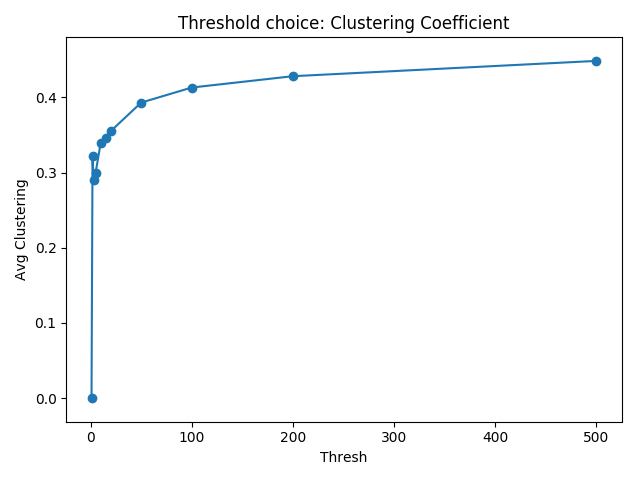
\includegraphics[width=1.\textwidth]{images/thresh_vs_avg_clustering.png}
        \caption{Clustering Coefficient vs. Threshold Size}
    \end{subfigure}
    ~
    \begin{subfigure}{0.4\textwidth}
        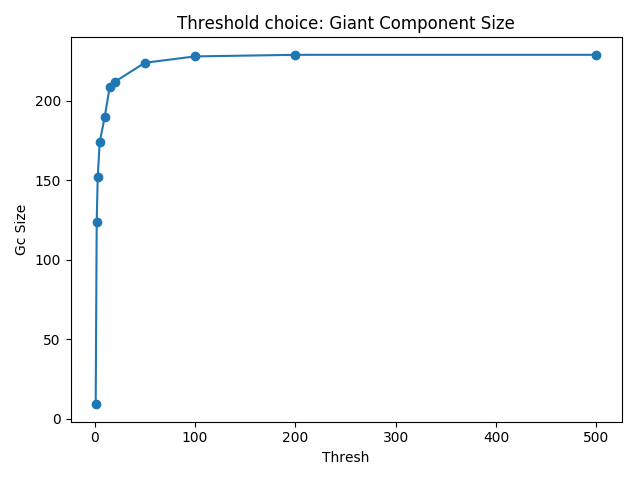
\includegraphics[width=1.\textwidth]{images/thresh_vs_gc_size.png}
        \caption{Giant Component Size vs. Threshold Size}
    \end{subfigure}
    \caption{Comparing threshold size effect on clustering coefficient and giant component size in order to determine the ideal threshold size.}
    \label{fig-threshold-size}
\end{figure*}

\subsubsection{Nodes and Edges}
Network nodes constitute each character identified in the set of found named entities. These were referenced against online resources to ensure proper coverage of the characters in the book. Edges in the book represent a co-mention between two entities in the text. A threshold number of tokens (words) under which the number of tokens between the mention of one entity and another determines if an edge is established. If the edge already exists, the weight is updated by adding `1' to the current weight value. The current entity $i$ is only matched with proceeding entities $j$ within this threshold. Once no match is found, the next available entity is checked for proceeding matches.

The threshold number of tokens is determined by a semi-objective measure of the effect of the threshold length on the average clustering coefficient and the giant component size (see Figure \ref{fig-threshold-size}). The intuition behind the use of these metrics is that we choose the minimum threhold length required to produce a large giant component and ample enough clustering best capturing the highly connected nature of characters in the novel. Our chosen threshold is 50 tokens.

\subsubsection{Section Snapshots and Modeling Recency}
One of the major considerations of our analyses concerns the ordering of sections. The book does not follow a chornological ordering with contiguous secitons potentially taking place anywhere within the time range of the book. However, the book Elegant Complexity \cite{carlisle_2007} provides a chronological ordering of sections. To perform a comparison of these two orders (`chronological' and `'booktime'), we constructed a timelapse of graph snapshots that represents the aggregate graph structure up to the current section in the given ordering. 

Regardless of the ordering, the graph at the end of each sequence will be identical. To model the differences in exposure to narratives and characters between the two orderings, we perform a decay mechanism of the weights of the graph. At each section, the corresponding graph snapshot's weights are mapped through a decay function developed orginially by psychologist Hermann Ebinghaus dubbed a `forgetting curve'. This curve is as follows:


\begin{equation}
    R = e^{\frac{-t}{(10000*s)}}
\end{equation}


Here $R$ represents the memory retention. $t$ represents the time, which we measure using the number of tokens per section. $s$ represents memory stability. The exponent is scaled by $\frac{1}{10000}$ to ensure reasonable memory retention values between $0$ and $1$. This approach enables us build a rough model the decaying memory of a reader to the narrative and character exposure differences between `chronological' and `booktime' section orderings.
